\clearpage
\section{Close proximity detection and\\ rover navigation}

The close proximity system consists of two main components, which are the readings from the ultrasonic sensors and the control of the rover using the motor controller. The ultrasonic sensors return distance measurements to the programme that then determines the optimal direction according to some thresholds and parameters.

\begin{figure}[H]
	\centering
	\begin{subfigure}[H]{0.4\textwidth}
		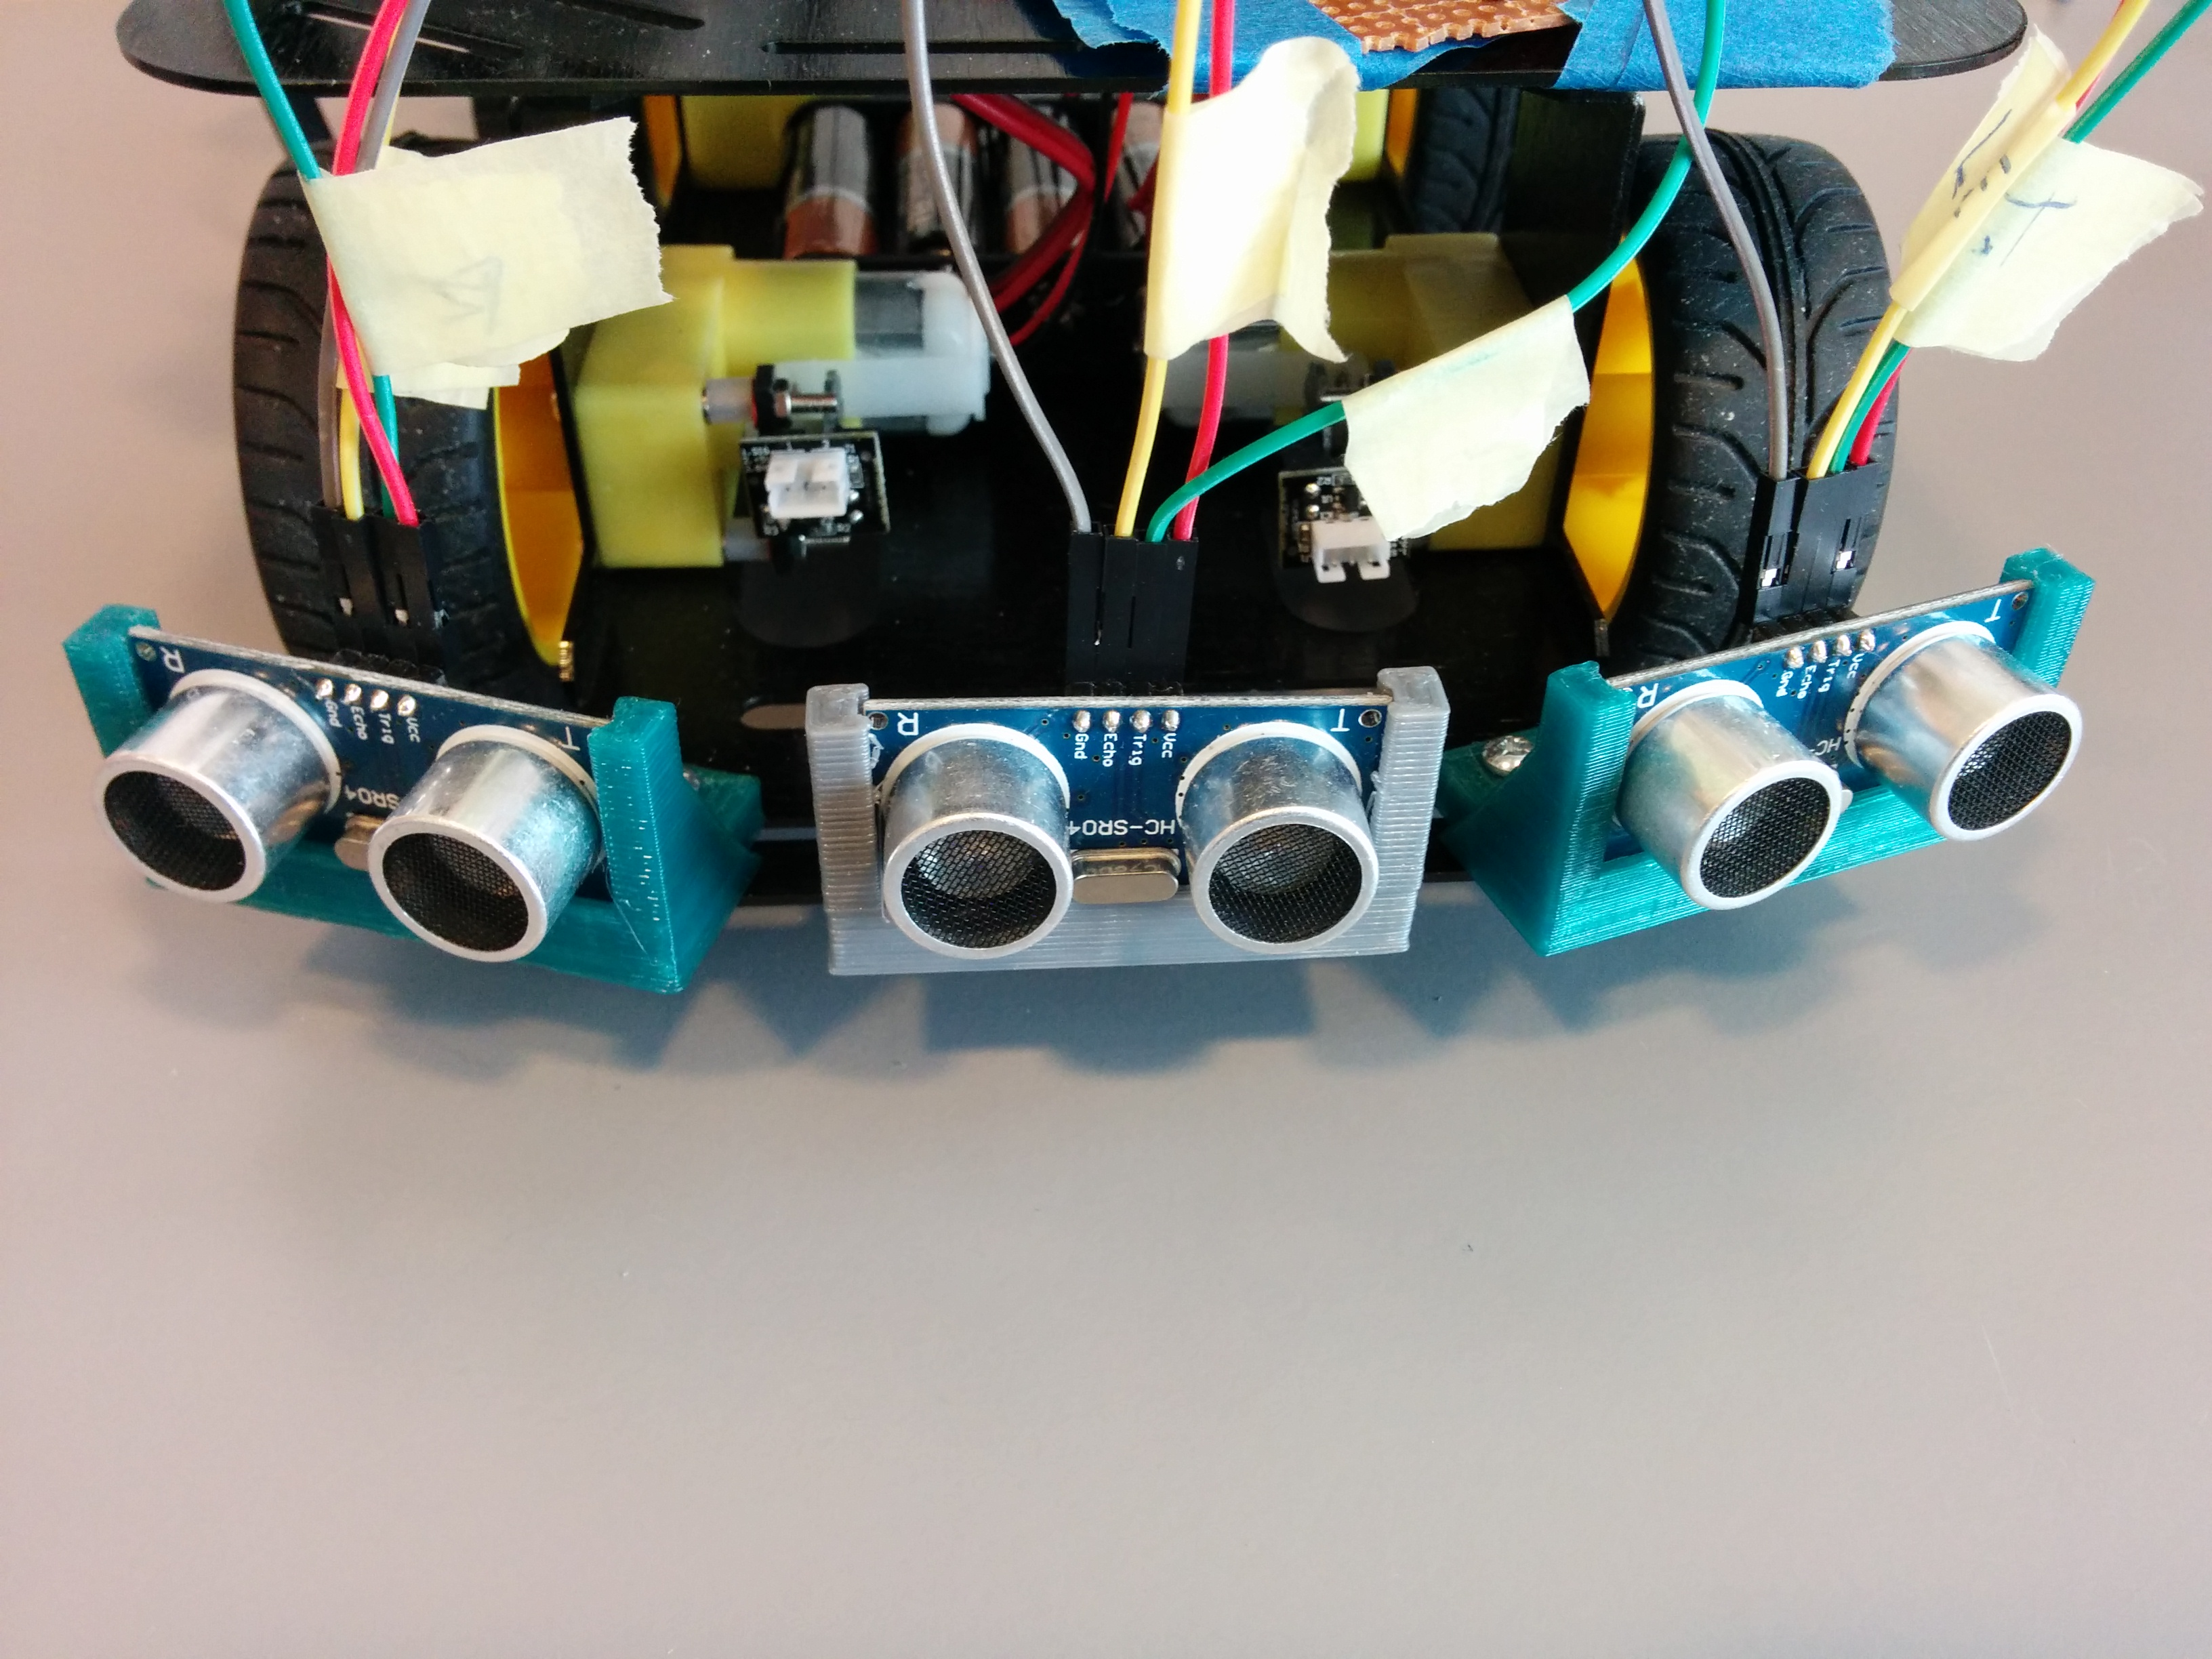
\includegraphics[width=\textwidth]{images/mounted_ultrasonic_sensors.jpg}
	\end{subfigure}%
	\quad
	\begin{subfigure}[H]{0.4\textwidth}
		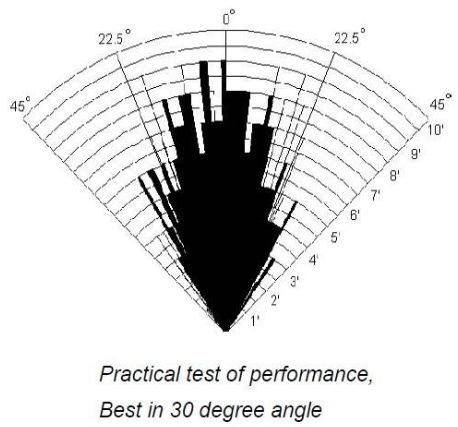
\includegraphics[width=\textwidth]{images/hcsr04angle.png}
	\end{subfigure}
	\caption{The enclosures used to mount the ultrasonic sensors on the chassis}
\end{figure}

The vision of the rover, which relies on the distance measurements from the sensors above, is currently limited to three different measurements. This unfortunately results in some blind spots between the ultrasonic sensors.
The ultrasonic sensor performs best at a $30\deg$ reading angle. This angle helps determine the area of which the ultrasonic sensor can read upon. The larger the angle, the less of a blind spot there will be between two ultrasonic sensors, depending on how they are mounted on the rover.\cite{hcsr40datesheet}.

\clearpage
\lstinputlisting[firstline=128, lastline=156, title=main, language=Python]{../code/autonomous-rover/obstacle-avoidance.py}

The core idea behind the current algorithm, is that per loop of the main code, the three ultrasonic sensors mounted on the front of the vehicle all gather three separate measurements. Then afterwards the measurements are compared in three different statements that will determine the direction. If the distance recorded by the left facing ultrasonic sensor is less than the threshold distance set as the variable \textit{avoid\_at}, the rover will then turn towards the right for the amount of seconds that the \textit{turn\_time} variable is set to. The same thing applies to the ultrasonic sensor faced to right, but instead the rover turns to the left when the threshold is exceeded.
If the threshold distance is exceeded at the center ultrasonic sensor, it determines whether the optimal path is to turn left or right depending on which direction has the largest distance measurement. This means that if an object is detected by the center ultrasonic sensor, the rover will then determine whether the distance measured to the left is greater than the distance measured to the right. The rover will then turn in the direction in which the distance measurement is greatest, since this theory means that the rover will have a longer distance until the rover meets an object.

%getdist()
\lstinputlisting[firstline=31, lastline=49, title=getdist(), language=Python]{../code/autonomous-rover/triple-ultrasonic-test.py}

At the start of the navigation loop seen in the \textit{main} code, the \textit{getdist()} function i run three separate times with different arguments, measurements are gathered every 200ms, where the datasheet recommends a measurements cycle of at least 60ms. The arguments are clearly labelled to help determine what measurement is coming from what ultrasonic sensor.
